\chapter*{{\color{red}Samenvatting}} %Ongenummerd hoofdstuk
\thispagestyle{empty} %Geen paginanummer deze pagina
\backgroundsetup{contents=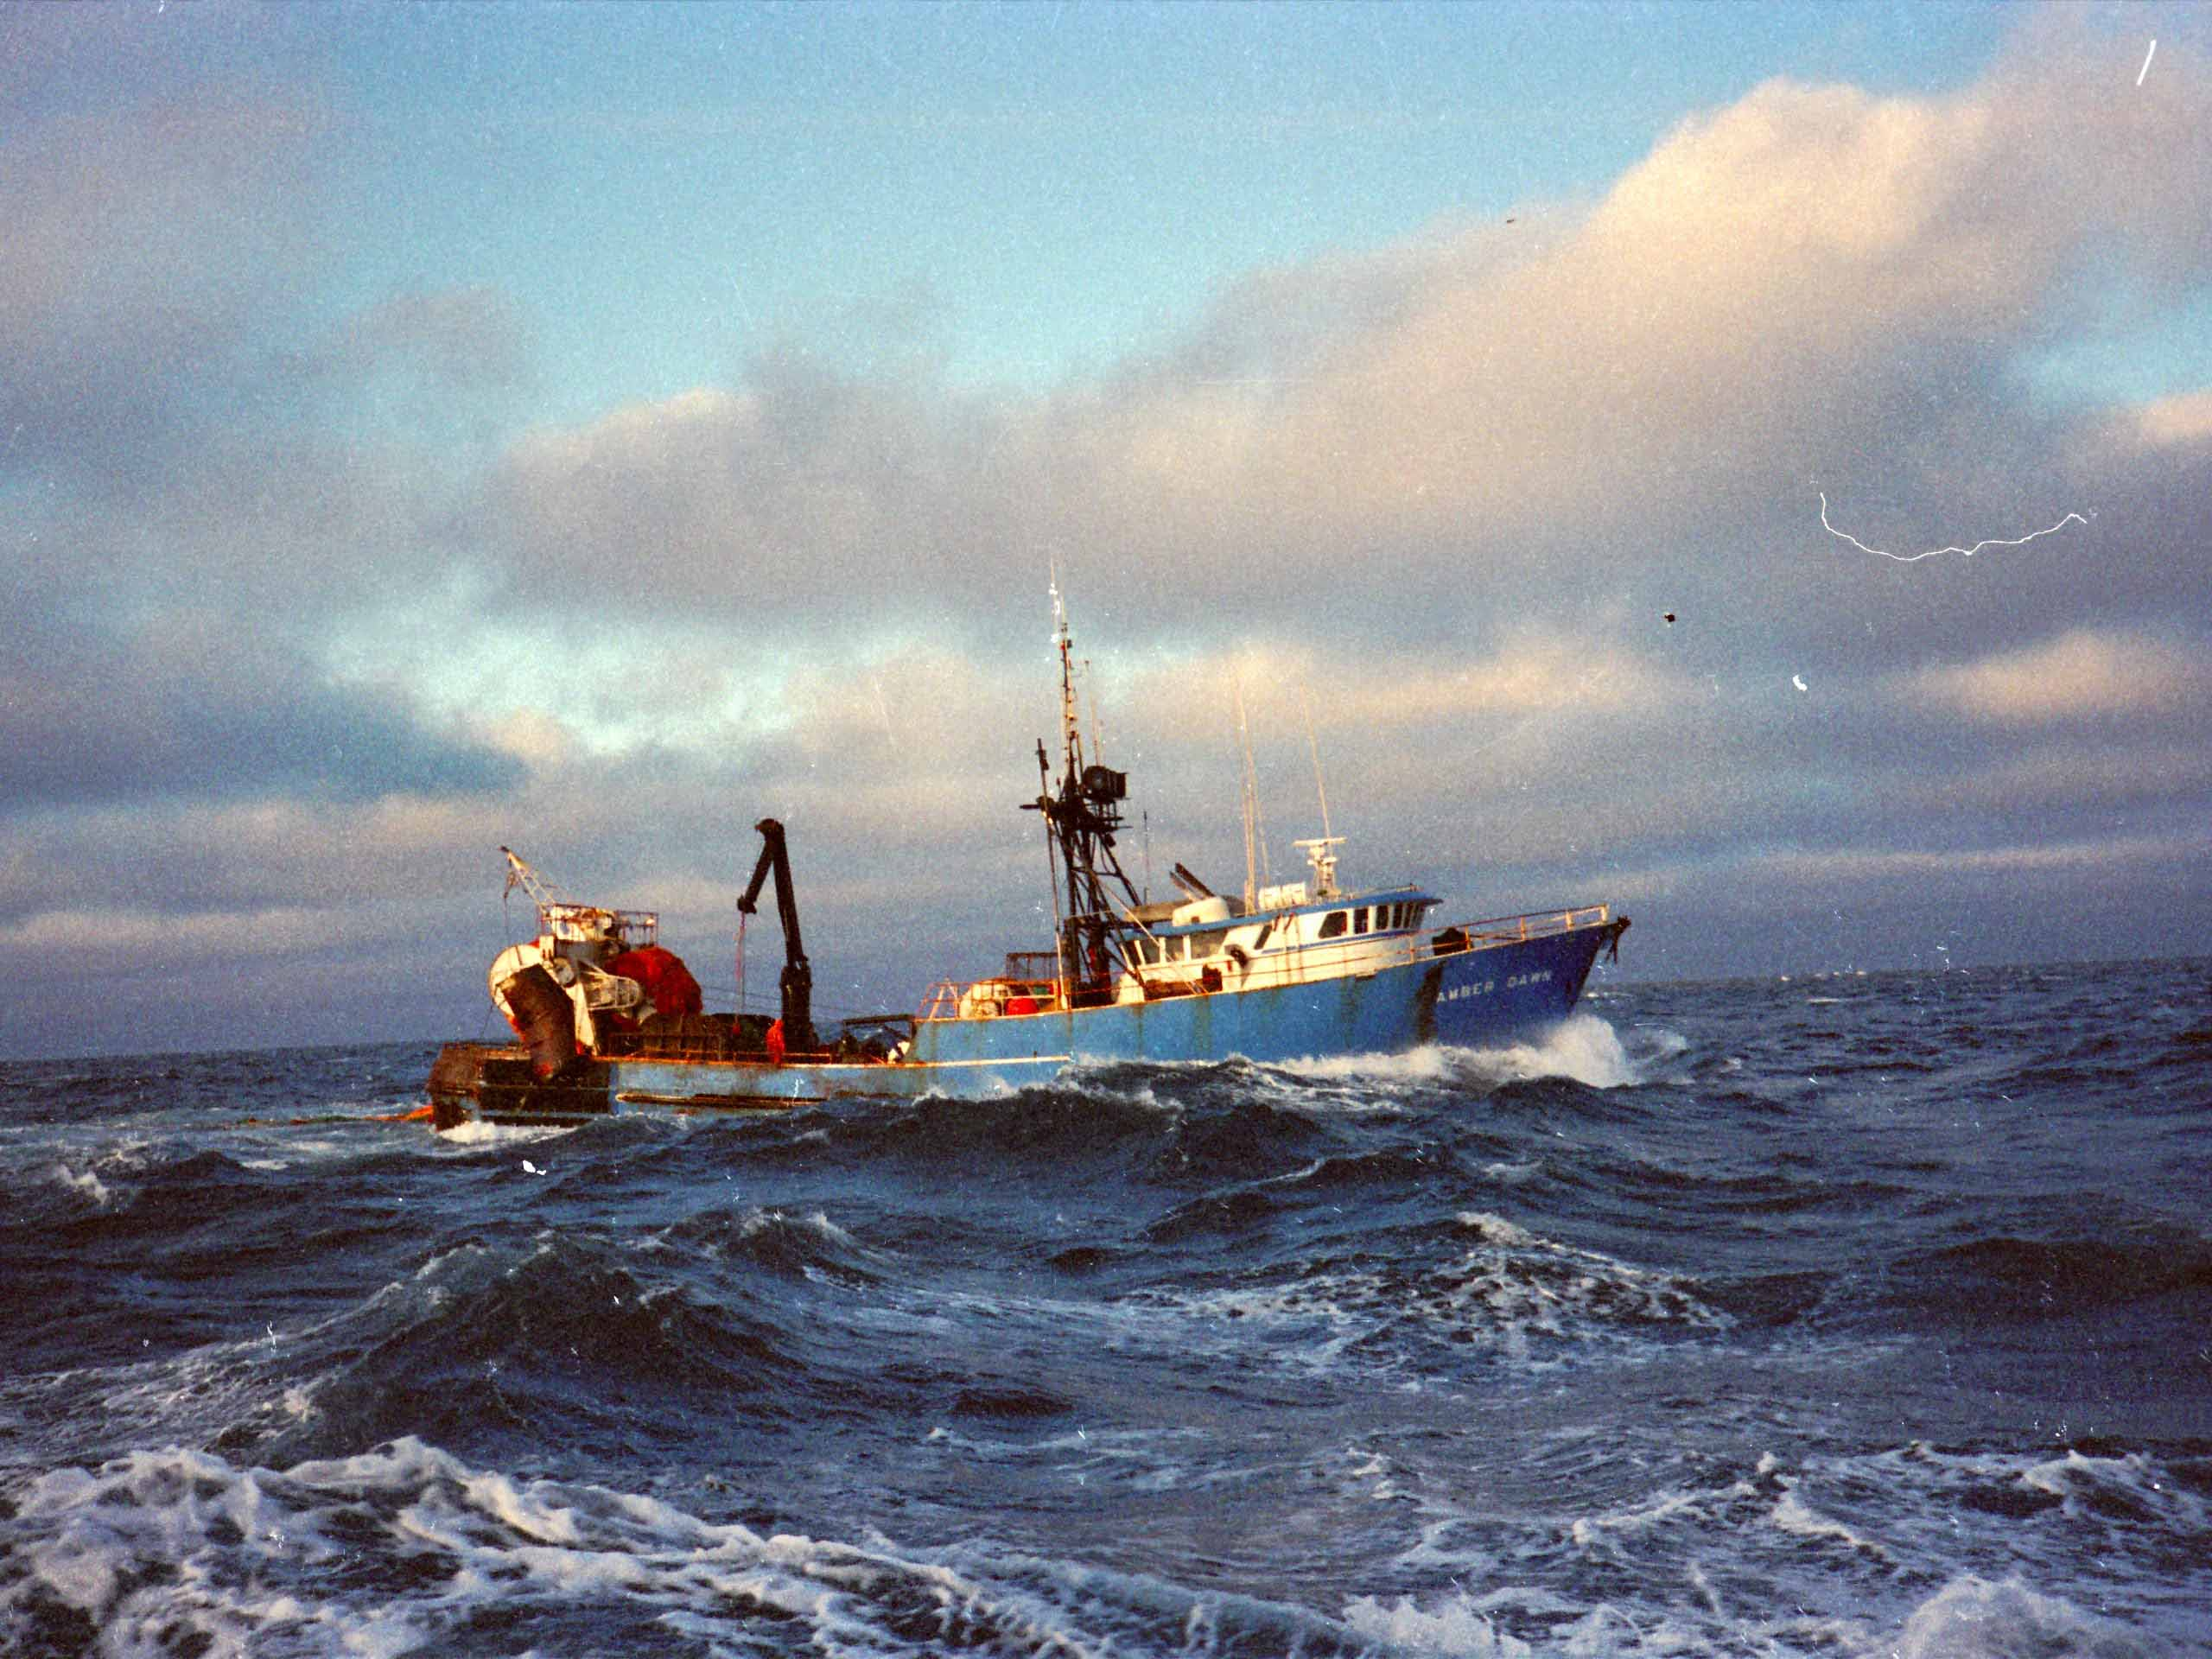
\includegraphics{BGbootALs},angle=0,scale=0.47,opacity=0.50,hshift=-634} %Instellingen voor achtergrondafbeelding
\BgThispage %Achtergrond deze pagina
\lipsum[1-4]









\begin{comment}
Een zakelijk rapport begint altijd met een (management)samenvatting. De belangstellende maar vaak gehaaste lezer moet snel weten waar het rapport over gaat en in welk kader het geschreven is, hoe het onderzoek is opgezet, wat de belangrijkste bevindingen zijn, de belangrijkste conclusies, aanbevelingen (adviezen) en (eventuele) financiële implicaties. Het is belangrijk dat de samenvatting de rode draad van je rapport toont13. Die rode draad is dan de basis voor je presentatie.
\end{comment}